\documentclass{article}
\usepackage{geometry}
\usepackage{graphicx}
\usepackage{setspace}

% Path to graphic images
\graphicspath{ }

% Title
\title{Wifi Connected Chess Boards \\ \large Feasibility Report Part 2}
\author{Nick Kraus, Kyle Jameson, Maurice Wallace, Mark Mauriello}
\date{\today}

% Margins
\geometry{letterpaper, portrait, margin=.75in}

\doublespacing

\begin{document}

\maketitle

%-----------------------
%		Hardware	
%-----------------------

\section*{Hardware}

\subsubsection*{Embedded System}
\indent

We have received many of the separate hardware sections and have connected them to the microcontroller for testing. We have successfully interfaced between the PSoC development board and stepper motor driver board, and using an external power supply were able to drive the stepper motors. The stepper motor drivers are very simple to interface to the microcontroller with very few components which will be required for the final hardware. We began to interface a character lcd display but encountered issues when too high of a voltage was accidentally connected to the back-light pin. Luckily we were able to make some discoveries about the lcd module before it became permanently damaged. It appears that the lcd module we previously had uses a driver ic which is incompatible with the PSoC's firmware digital module; though we were able to get the hardware into what appeared to be a working configuration the lcd never displayed the correct characters. The magnetic system was also tested by checking to see that the small neodymium magnets would trip the reed switches at a reasonable distance and that an electromagnet would be able to move the neodymium magnets at a similar distance.

\indent

Work has begun on developing a schematic for the final hardware. This includes creating schematic symbols for all of the parts and reading the datasheets of the parts which will be used in the final hardware. Reference schematics have been found for the microcontroller and the datasheets for the lcd display, stepper motor drivers, and wifi module all discuss how to interface to them. Once all the symbols have been drawn up the schematic can be completed and reviewed.

%-----------------------
%		Software	
%-----------------------

\section*{Software}

\subsubsection*{Microcontroller Firmware}
\indent

For this project, we dove deeper into the firmware of the micro controllers by creating and testing many of the functionalities that the firmware can provide. For the PSoC we went through the documentation of pin manipulation. First the pin or pins that we wished to use were represented in our virtual design and model of the micro controller in our IDE. We ran tests that included frequency manipulation of the LED pin. With that we learned how to time the writing to pins. Using a delay function and n io write function we were able to control the voltage of an output pin. This came in handy when we tested the stepper motor. After reading the documentation of the driver used for the stepper motor, we had the correct connections and firmware to guide the motor. The stepper motor was controlled by driving two out of a set of four pins high at certain intervals. By determining the delay between the writes, we could determine the speed of the stepper motor. The fastest the motor could spin was when the delay was between 1.5 and 2 milliseconds. The other piece of firmware that we tested and learned about was for an LCD screen. This LCD screen had its own documentation and function calls in code that we read and learned about. To make sure that the firmware and hardware would actually work we decided to take an example that cypress had. This firmware worked properly because it was an example, yet the LCD did not work even though the hardware was connected properly. Thus it was determined the LCD driver was not compatible with the firmware/hardware that was implemented. As of right now we are able to control the pins of the micro controller, the drivers to the stepper motor, and understand the firmware for the an LCD screen that would properly work.

\subsubsection*{WiFi Module Firmware}
\indent

The ESP8266 WiFi module was successfully able to interact with the UART bus in order to obtain access to a created wireless network. To achieve this, we introduced a software called CoolTerm, a serial port terminal application that is used for exchanging data with hardware connected through serial ports. With proper documentation pertaining to the WiFi module, we used the serial terminal to attempt to connect to a TCP server created through Python. The serial terminal available allows us to search for potential connections and join them, provided we know the credentials. The terminal also allows a means to connect to multiple connections as well as connect to a remote TCP server with the corresponding IP address and port. With access to the server, we will have the ability to send data based on a byte size of our choosing to be received by the server. We were also able to receive data on the wifi module sent from a TCP server, which displayed properly in the serial terminal.

\indent

We are capable of reprogramming the firmware on the WiFi module. Our next step is to reference the modules documentation pertaining to creating our own custom firmware.

\centerline{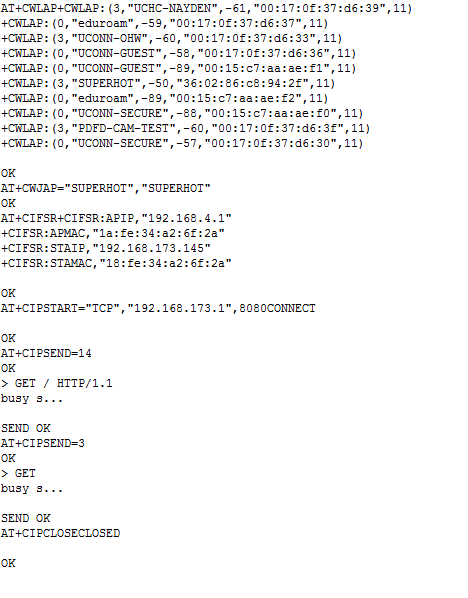
\includegraphics[scale=.5]{SerialMonitor}}

\begin{center}
The serial monitor and data sent from the ESP8266 WiFi Module.
\end{center}

\subsubsection*{Server}
\indent

We went through the process of setting up a laptop to do two things. First, the laptop broadcast a WiFi network for the ESP8266 WiFi module to connect to, and second, the laptop hosted a simple Python server for handling HTTP GET requests. Through these GET requests, we were able to determine whether or not the WiFi module was successfully connecting. However, the Python server was running into some issues sending responses back to the WiFi module. Also, the server was only logging the bad (HTTP 400) requests, and not the good (HTTP 200) requests. So we used another piece of software called Hercules to more accurately determine what, if anything, the module was sending to the server. With Hercules, we found out that the syntax of our raw GET requests was incorrect, but we were able to send raw TCP data successfully. So we determined that the server was receiving data from the module, but not through a Python server, and we need to reform our request syntax to be successful herein.

\centerline{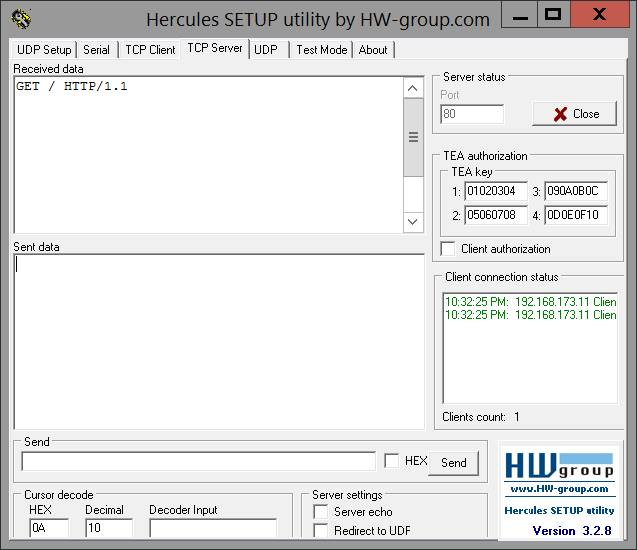
\includegraphics[scale=.5]{Hercules}}

\begin{center}
The hercules program receiving a tcp message.
\end{center}

\centerline{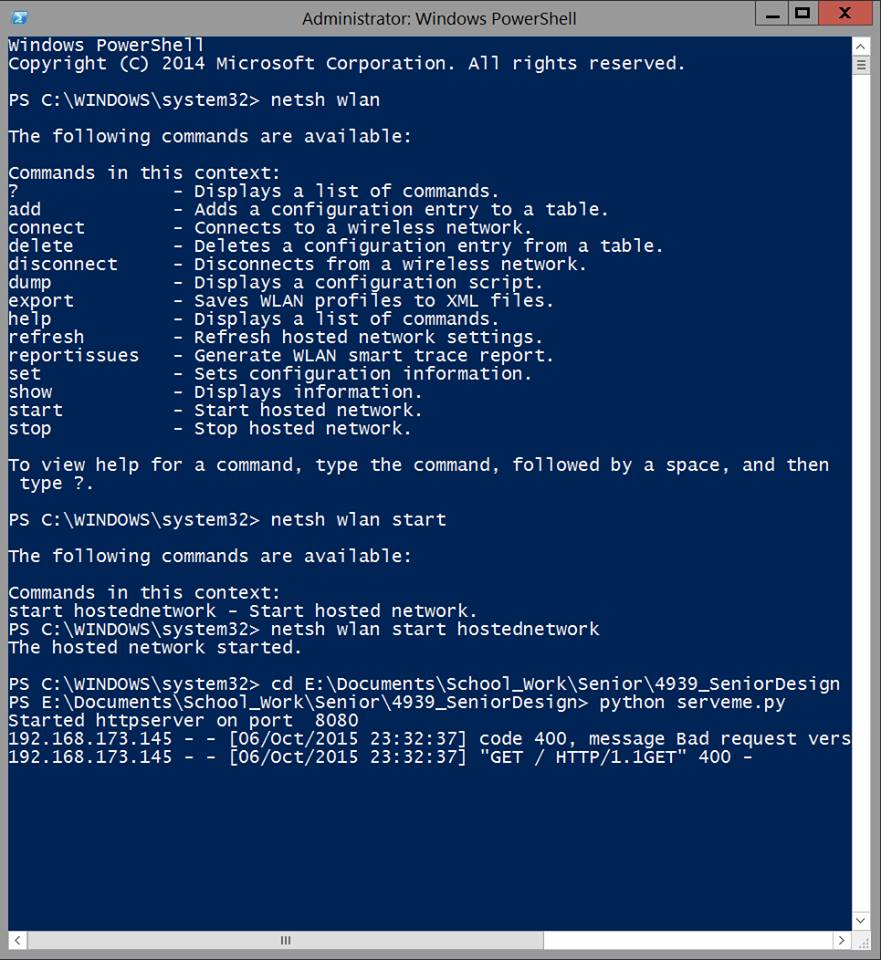
\includegraphics[scale=.3]{Python}}

\begin{center}
The python server with a failed http request.
\end{center}

\end{document}